\chapter{Introduction}
\label{chp:introduction}

% \begin{quotation}[]{Poul Anderson}
% I have yet to see any problem, however complicated, which, when looked at in the
% right way, did not become still more complicated.
% \end{quotation}

Mutation testing is a technique to better guide the testing process~\cite{DEMILLO:1978:1, JIA:2011:1}. The idea consists in performing program transformations to introduce artificial bugs to check whether the existing test suite is capable of detecting them. However, the costs of using mutation testing are usually high. Two kinds of mutants contribute to increasing such costs: equivalent and duplicated mutants. Equivalent mutant is a mutant that has the same behavior as the original program \cite{BUDD:1982:1, JIA:2011:1, MADEYISKI:2014:1}. So, this mutant is useless. A duplicated mutant, on the other hand, has the same behavior as other mutant \cite{PAPADAKIS:2015:1, KINTIS:2017:1}. This way, one of them is useless. 

Figure~\ref{fig:background} illustrates one equivalent mutant and two duplicated mutants. 
Mutant \textit{M2} introduces a post increment to a local variable (\texttt{a++}). 
Notice that this introduction does not change the behavior when compared to the original program since the increment would happen after the function returns and \texttt{a} is a local variable. 
In this sense, \textit{M2} is useless. Mutant \textit{M3} removes the right-hand side of the arithmetic expression, yielding \texttt{fieldId\_0 = fieldId\_1}. 
Mutant \textit{M5} replaces the \texttt{+} operator by \texttt{*}, yielding \texttt{fieldId\_0 = fieldId\_1 * 1}. 
These mutants have the same behavior and thus are duplicated. Therefore, either \textit{M3} or \textit{M5} is useless.

\begin{figure}[h]
\begin{center}
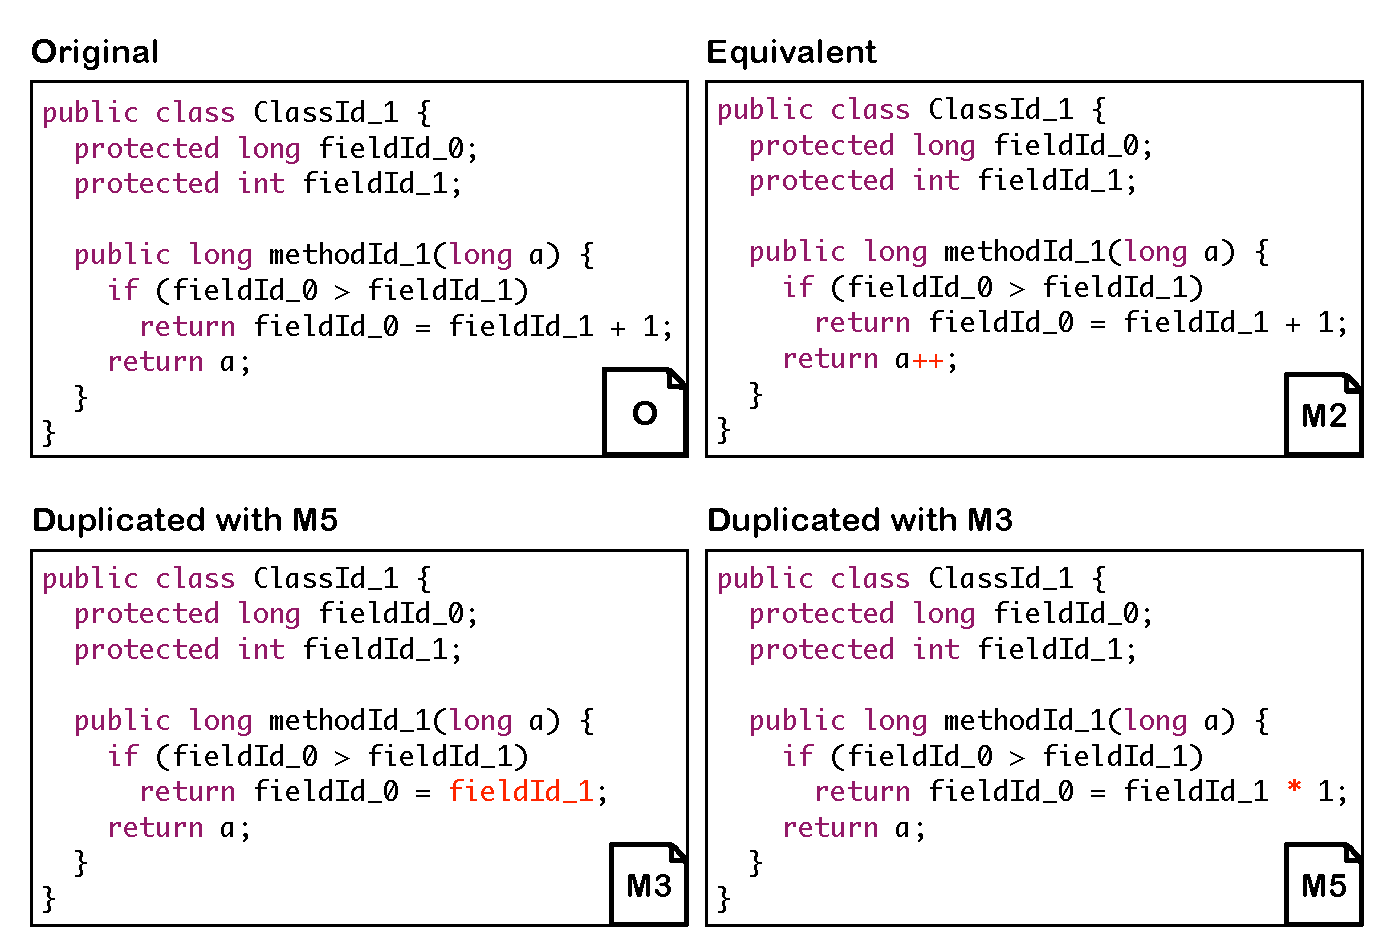
\includegraphics[scale=0.5]{images/Background.pdf}
\caption{Original program and three mutants.}
\label{fig:background}
\end{center}
\end{figure}

Previous work~\cite{MADEYISKI:2014:1} reported that the rate of equivalent mutants might lie between 4\% and 39\%. 
In addition, manually checking mutant equivalence is error-prone (people judged equivalence correctly in about 80\% of the cases~\cite{ACREE:1980:1}) and time consuming (approximately 15 minutes per equivalent mutant~\cite{SHULER:2013:1}). 
Recently, duplicated mutants have been discussed and tackled. 
Researchers reported 21\% of duplicated mutants in their empirical study~\cite{KINTIS:2017:1}.

In this work, we introduce a strategy to help with identifying rules capable of avoiding useless mutants. 
To use the strategy, we need a set of programs as input. 
In addition, for each program in this set, the strategy also needs a green test suite and a set of mutants derived from the program. 
The strategy then runs every test against every mutant and yields equivalent and duplicated mutants candidates. 
Our strategy is flexible in the sense we can instantiate it with different programs and their respective test suites. To generate the mutants, we can instantiate the strategy with different mutation testing tools.

% As you can see, our strategy works similarly to a normal mutation analysis.
% But we use the test suite itself to identify useless mutants.
% It is based on three major modules that are flexible to instantiate one or more tools for each one of the modules.

% \begin{itemize}
%     \item The program input.
%     \item The mutants.
%     \item The test suite.
% \end{itemize}

To classify the mutants as equivalents or duplicated, the strategy proceeds as follows. 
Given a program \textit{P}, when its test suite \textit{T} is executed in a mutant \textit{M} and it does not have any failing test case, the strategy classifies \textit{M} as an equivalent mutant candidate. If two mutants \textit{M$_i$} and \textit{M$_j$} have the same non-empty set of failing test cases in \textit{T}, the strategy classifies \textit{M$_i$} and \textit{M$_j$} as duplicated mutants candidates. 

To evaluate our strategy, we instantiate it with programs automatically generated by the \jdolly{} program generator~\cite{SOARES:2013:1}. 
\jdolly{} exhaustively generates programs up to a given scope. 
It encodes a metamodel for Java and uses the Alloy specification language \cite{alloy-book} to find possible solutions, which are translated into Java programs.
The user can specify constraints to guide \jdolly{} to generate programs in a given scope.
In our work, we set \jdolly{} to generate \AnalyzedPrograms programs with few Java constructs. 
This reduced Java scope makes the task of deriving rules to avoid useless mutants easier. 

As our programs did not have any test suite, we use \randoop{}~\cite{PACHECO:2007:1} to automatically
generate unit tests for the classes and methods received as parameters within a time limit.
A unit test generated by \randoop{} typically consists of a sequence of
method and constructor invocations that create and mutates objects with random values and a JUnit assertion.

%\todo{Last but not least}, 
%we choose to work in Java since it is widely used by practitioners and forms the subject of most of the recent research papers.
To generate the mutants, we instantiate three of the most used Java mutation testing tools, i.e., \mujava{}~\cite{OFFUTT:2005:1, OFFUT:2006:1}, \major{}~\cite{JUST:2011:1}, and \pit{}~\cite{PIT:2017}.
These tools, in addition to being the most used in previous research, bring different mutation operators as well as different approaches to mutant generation: source code mutation (\mujava{}), byte code mutation (\pit{}), and compiler-integrated mutation (\major{}).

The three mutation testing tools generated 4,999 mutants. 
The strategy classified 963 as equivalent and 1,332 as duplicated.
By analyzing the results, we observe we could avoid many mutants classified as useless in case we perform an analysis of the context in which the mutation is applied.
We can retrieve this context by navigating throughout the Abstract Syntax Tree (AST) or by using \textit{def-use} analyses.
So, the output of our strategy is important because it enables us to derive rules to avoid the generation of these mutants. 

In particular, after manually analyzing the output, we derived \NumberOfIdentifiedHeuristics rules. 
To the best of our knowledge, \NumberOfNewHeuristics out of \NumberOfIdentifiedHeuristics are first introduced in this work.
%A rule is defined as a triple ($terms$, $transformations$, $constraints$).
%This small set of information, which we better explain each part in Chapter \ref{sec:rules}, is sufficient to predict some useless mutants and thus prevent them from being generated.
To evaluate the effectiveness of our rules on reducing costs, we have implemented a subset of them in the \mujava{} tool. 
We execute the tool using classes of well-known projects such as \textit{ant}, \textit{bcel}, and \textit{commons-lang}. 
As results, we reduce the number of mutants by almost 13\% on average, demonstrating potential. 
One might wonder that this number is low when compared to related work. 
However, these results are promising because differently from previous work~\cite{PAPADAKIS:2015:1, KINTIS:2017:1, BALDWIN:1979:1, OFFUT:1996:1, OFFUT:1997:1, VOAS:1997:1, HIERONS:1999:1, GRUN:2009:1, SHULER:2010:1, SHULER:2013:1, SHULER:2009:1}, we do \textit{not} generate, compile, and analyze whether the mutants are useless or not. 
Instead, we avoid them: our rules are capable of discarding such mutants right before their generation. Also, we can derive more rules in case we set our strategy with more complex Java programs. Last but not least, we have implemented only a subset of our rules. We focused on rules that do not need \textit{def-use} analyses. 

We also calculated the execution time of our rules to better understand whether pre-analyzing and avoiding mutants is faster than generating useless mutants and checking whether they are indeed useless or not. Despite the overhead introduced by our rules, the payoff amount is higher than 12\% for all projects we considered in this work and reached almost 20\% in two projects.

%An important issue arises when we add an overhead before generating mutants. Would it be better to generate the useless mutants and then detect them instead of doing a pre-analysis to avoid them? After all, although we avoid some mutants, these rules would be executed every time that mutation operator is selected. To understand this trade-off, we calculate the execution time of the tool either without the rules and with the rules embedded. To our surprise, despite the overhead introduced by our rules, the payoff amount is higher than 12\% for all projects and reached almost 20\% in two projects which we analyzed. That is, the cost of running all rules is offset by the decrease in the number of mutants to generate and compile.

This work presents the following contributions:

\begin{itemize}
    
    \item A strategy to help with identifying rules to avoid equivalent and duplicated mutants (Chapter~\ref{sec:strategy});
    
    \item We introduce \NumberOfNewHeuristics new rules to \textit{avoid} the generation of equivalent and duplicated mutants (Chapter~\ref{sec:rules});
    
    \item We provide a \mujava{} implementation embedded with \NumberOfImplementedHeuristics implemented rules (Chapter~\ref{sec:implementing}).
    
    \item An empirical study to evaluate our rules. In particular, we avoid almost 13\% (on average) of useless mutants in classes of well-known projects such as \textit{ant}, \textit{bcel}, and \textit{commons-lang} with a payoff amount higher than 12\% for all projects in the execution time (Chapter~\ref{sec:implementing});
    
\end{itemize}


%\section[Motivation  (Why to Automate CR Assignment?)] {Motivation (Why to Automate \ac{cr} Assignment?)}
%\label{sec:intro-motivation}
%
%\section{Problem Statement}
%\label{sec:intro-problem-statement}
%
%\section{Overview of the Proposal}
%\label{sec:intro-solution}
%
%\section{Research Methodology}
%\label{sec:intro-methodology}

%This research design of this thesis is based on a multimethod
%approach~\citep{Hesse-Biber2010}. Such approach combines two or more
%quantitative (or qualitative) methods in a single study, such as a survey and an
%experiment~\citep{Hesse-Biber2010}. Multimethod must not be confused with mixed
%method. In this last, methods for both qualitative and quantitative types of
%research are applied in a single study. On the other hand, multimethod studies
%combine different methods for a single research type.
%
%When applying a multimethod approach, the triangulation is used to consolidate
%the results from the different methods, considering, however, that the same
%research question(s) was/were investigated in these methods. As a consequence,
%the triangulation of methods enhances the conclusions and completeness of the
%study, bringing more credibility to the research
%findings~\citep{Hesse-Biber2010}. \figref{fig:research-methodology-thesis} shows
%the multimethod research design applied in this thesis.
%
%\begin{figure}[h]
%\centering
%  \caption[Research methodology.]{The research methodology applied for this
%  thesis.}
%  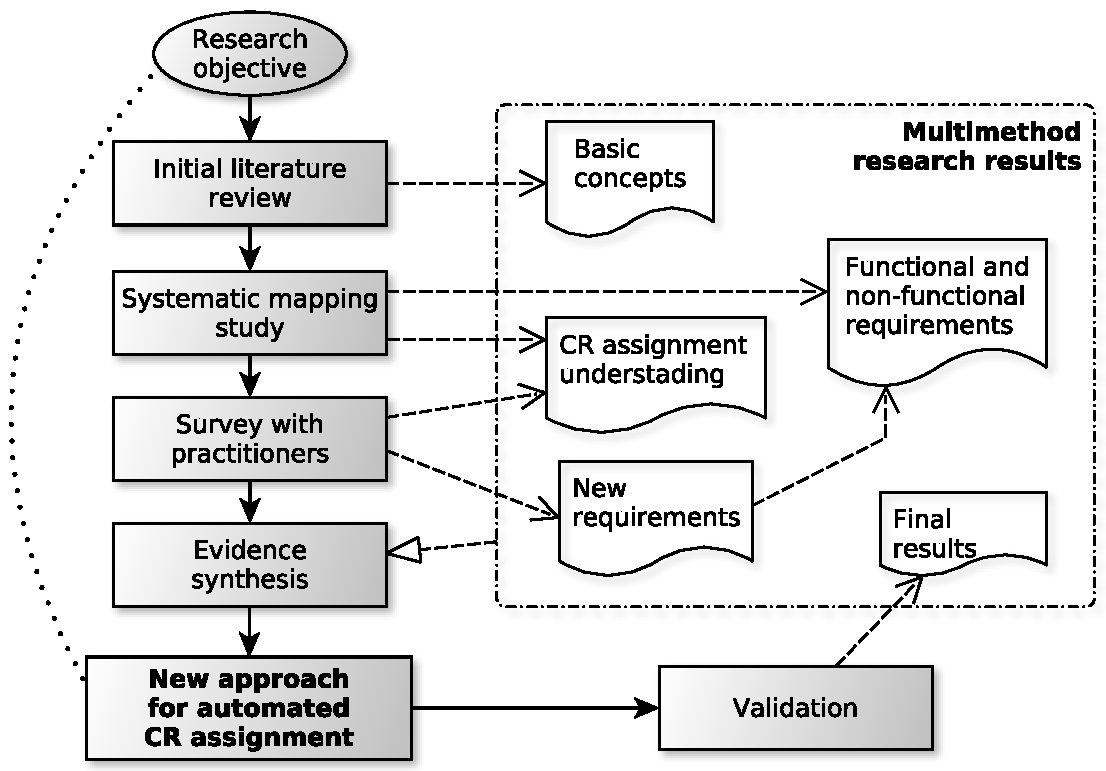
\includegraphics[width=\columnwidth]{images/research-methodology-thesis.pdf}
%  \footnotesize{Source: Made by the author.}
%  \label{fig:research-methodology-thesis}
%\end{figure}
%
%The design started by stating the research objective, which we defined in
%\secref{sec:intro-problem-statement}, and performing the initial literature
%review. This last provided the basic concepts and understanding of the area.
%Then, a systematic mapping study and a questionnaire-based survey were
%conducted. These two gathered detailed information on our research topic.
%Indeed, both of them were used to understand the key aspects of \ac{cr}
%assignment and identify the set of requirements to automate the assignments. In
%the evidence synthesis step, these results were detailed and organized in order
%to formulate the approach to automate \ac{cr} assignments, which was constructed
%in the next step. Finally, the research design states the validation of the
%proposed approach.

%\section{Out of Scope}
%\label{sec:intro-outofscope}
%As the proposed approach is part of a broader context, a set of related aspects will be left out of its scope. Thus, the following topics are not directly addressed in this thesis:
%
%\begin{enumerate}
%  \item \textbf{Tools for \ac{cr} management.} We are addressing
%  a specific aspect of \ac{cr} management, which is the \ac{cr} assignment
%  activity. Thus, it is out of scope of this thesis to provide a
%  complete solution for \ac{cr} management. Instead, we are planning to
%  implement standalone software which will be able to integrate with the
%  most well known tools for \ac{cr} management, such as Mantis, Bugzilla, and
%  Trac, providing a service to leverage the automation of \ac{cr}
%  assignments.
%  
%  \item \textbf{Software maintenance process.} Software maintenance involves
%  a set of activities aiming at implementing modifications in some software
%  project. These activities must be coordinated through a process so that the
%  maintenance can be successful. In Chapter 2, we discuss some of
%  these processes. However, in this thesis, we are not concerned with the
%  maintenance process itself. Actually, it should be transparent in our approach
%  to automate \ac{cr} assignment. Thus, it is out of scope of this
%  thesis to provide any process assessment for software maintenance beyond the
%  activity of \ac{cr} assignment.
%  
%  \item \textbf{\ac{ir} models.} Many models for \ac{ir} have been proposed for
%  different objectives, including the \ac{cr} assignment itself. However, due to
%  the broad availability of these models, it is out of scope of this thesis to
%  develop a new one. Instead, the \ac{ir} models with better performance,
%  identified through the systematic mapping study, were chose to be
%  integrated in our approach;
%  
%  \item \textbf{Rule-based expert systems.} Similar to \ac{ir} models,
%  rule-based expert systems have a long history of development. Thus, our
%  approach does not intend to develop a whole new system with this purpose.
%  Actually, we integrated in our approach the
%  Drools\footnote{\url{http://www.jboss.org/drools/}} expert system, which is a
%  mature tool that can be easily manipulated;
%  
%  \item \textbf{Mathematical formulations on NP-Complete problems.} We
%  understand that the problem of assigning \acp{cr} to software developers is in
%  the broad category of \emph{assignment problems}, which is well known to be
%  NP-Complete. Thus, could be formulated as such. However, the mathematical
%  formulations of the \ac{cr} assignment problem is out of scope of this thesis.
%  As well as finding an optimal solution on the context of NP-Complete problems
%  is also out of scope. The main reason for this is the human factors and
%  context variables that are involved in the assignment of \acp{cr}, which
%  make this problem hard to be computable. A mathematical formulation of the
%  \ac{cr} assignment problem is provided by~\citet{Rahman2009}.
%\end{enumerate}

%\section{Statement of the Contributions}
%\label{sec:intro-contibutions}

%\section{Organization of the Thesis}
%\label{sec:intro-organization}

